\cxset{style11/.style={
 chapter opening=any,
 chapter name=Chapter,
 numbering=arabic,
 number font-size=LARGE,
 number font-family=rmfamily,
 number font-weight=bfseries,
 number before=,
 number dot=,
 number after=,
 number before=\kern0.5em,
 number display=inline,
 number float=none,
 chapter display=block,
 chapter float=center,
 chapter font-family=rmfamily,
 chapter font-weight=bfseries,
 chapter font-size=LARGE,
 chapter before=,
 chapter after=,
 chapter color=black!90,
 chapter spaceout=none,
 chapter border-width=0pt,
 chapter border-style=none,
 chapter display=block,
 chapter float=center,
 number display=none,
 number color=black!90,
 title beforeskip=,
 title afterskip=,
 title before=,
 title after=,
 title font-family=rmfamily,
 title font-color=black!90,
 title font-weight=bfseries,
 title font-size=LARGE,
 title margin-left=0pt,
 title display=block,
 title float=center,
 chapter title width=\textwidth,
 chapter title align=centering,
 section afterindent=true,
 section align=left,
 section numbering=arabic,
 section numbering prefix=\thechapter.,
 section numbering suffix=\space,
 section indent=0pt,
 section font-family=rmfamily,
 }}
\renewsection\renewsubsection

\cxset{style11}
\chapter{\textit{Elements} II and Babylonian Metric Algebra, Introduction to Style Eleven}

The origins of Greek Mathematics, according to the Greeks is Egypt and according to J\"oran Friberg is Babylonia. This template is based on Friberg's book \emph{Amazing Traces of a Babylonian Origin in Greek Mathematics}. The book was published by World Scientific in 2007. The book size is $5.97\times8.88$ inches and uses a variety of fonts, with the main document font in Times. 

\medskip
\begin{figure}[ht]
\centering
\fbox{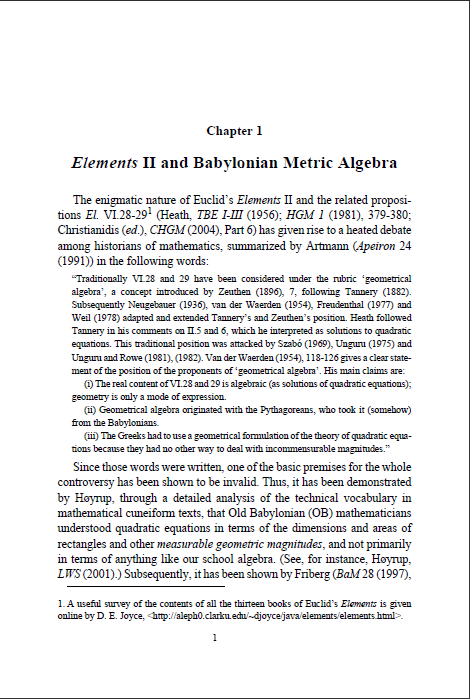
\includegraphics[width=0.65\textwidth]{./chapters/chapter11.png}}
\end{figure}
\lipsum[1]

\section{Indentation}

The book follows swedish traditional typography with the paragraphs following subheadings indented. This is achieved in the template using:

\begin{verbatim}
\cxset{section afterindent=true}
\end{verbatim}

\section{Images}
\indent Images and their captions follow a \latexe style and I am sure the book must have been styled using a \latexe xml clone as the book's pdf was produced with iText\footnote{\url{http://itextpdf.com/}}.

\begin{figure}[ht]
\centering
\includegraphics[width=0.8\textwidth]{greekmaths}
\caption{Extract from the \textit{Amazing Traces of Babylonian Influence in Greek Mathematics.} Note the styling of the caption.}
\end{figure}

\testsections

% reset for following chapters
\cxset{section afterindent=false}

